\documentclass{standalone}

\usepackage{tikz}
\usepackage{xcolor}
\usepackage{amsmath}
\usetikzlibrary{shadows}


\begin{document}

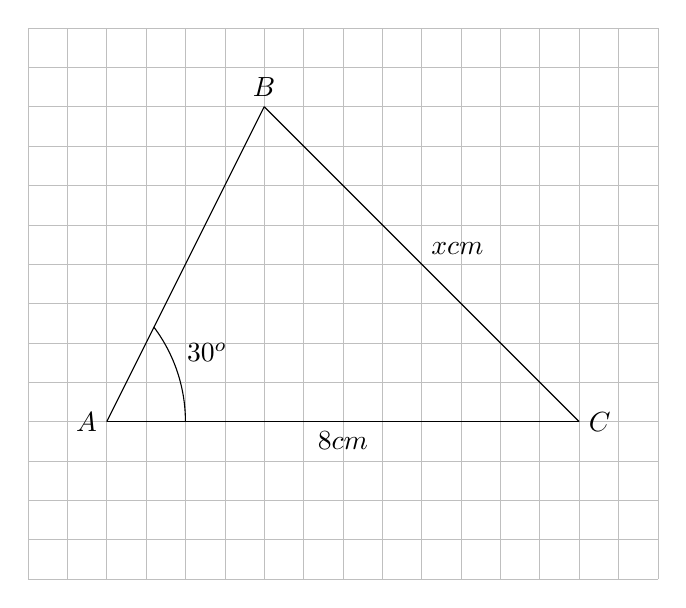
\begin{tikzpicture}
    \draw[step=0.5, lightgray, very thin] (-1,-2) grid (7,5);
    %\draw[dotted, <-stealth] (1,1) node[above=1pt] {$\mathbf{a}$} -- (3,3);
    %\draw[red,thick,dashed] (2,2) circle (10pt);
    %\draw (0,0) .. controls (0,4) and (4,0) .. (4,4);
    %\filldraw[red] (2,2) circle (3cm);
    %\coordinate (A) at (2,1);

    \coordinate[label=left:$A$] (A) at (0,0);
    \coordinate[label=above:$B$] (B) at (2,4);
    \coordinate[label=right:$C$] (C) at (6,0);

    \draw (A) -- (B);
    \draw (B) -- (C) node[midway, above right] {$x cm$};
    \draw (C) -- (A) node[midway, anchor=north] {$8 cm$};

    \draw (1,0) arc (0:37:2cm) node[midway, above right] {$30^o$};
\end{tikzpicture}

\end{document}
